\documentclass[10pt]{article}
\usepackage[margin=1.5in]{geometry}
\usepackage[utf8]{inputenc}
\usepackage{graphicx}
\usepackage{authblk}
\usepackage{titlesec}
\usepackage{svg}
\begin{document}

\title{ARM11 Project Final Report}
\author{C Group 03}
\affil{Andy Chen, HouWang Wong, Jeshuran Jebanesan, Jiaju Yang}

\maketitle

\section{Abstract}
This project aims to develop an ARM11 assembler that can decode basic ARM11 assembly language and translates it into binary machine code. The task is done in a two-pass algorithm: recording any symbol for branch instructions and storing them into a table in the first pass, and replacing these symbols with their corresponding value during the translation process in the second pass. In addition, a three-player chess game for a hexagonal 96-tile board is implemented as a C program extension, which includes the main board logic code and a chessboard GUI.
\section{Assembler}
\subsection{General structure}
For the assembler, a test-driven approach was taken, where the testing framework for the functions was designed first, and then the functions themselves were defined. From the development experience in the first half of the project, the fact that only a few function tests were performed before debugging stage would result in a long debugging time due to the difficulty of pinning down the problematic parts of the code.
As shown in Figure 1, the structure was divided into 4 main parts.
\begin{figure}
\centering
\begin{minipage}{.5\textwidth}
\centering
\includegraphics[width = \linewidth]{ Assembler_structure }
\caption{Assembler workflow chart}
\label{fig:Assembler_structure}
\end{minipage}\hfill
\begin{minipage}{.5\textwidth}
\centering
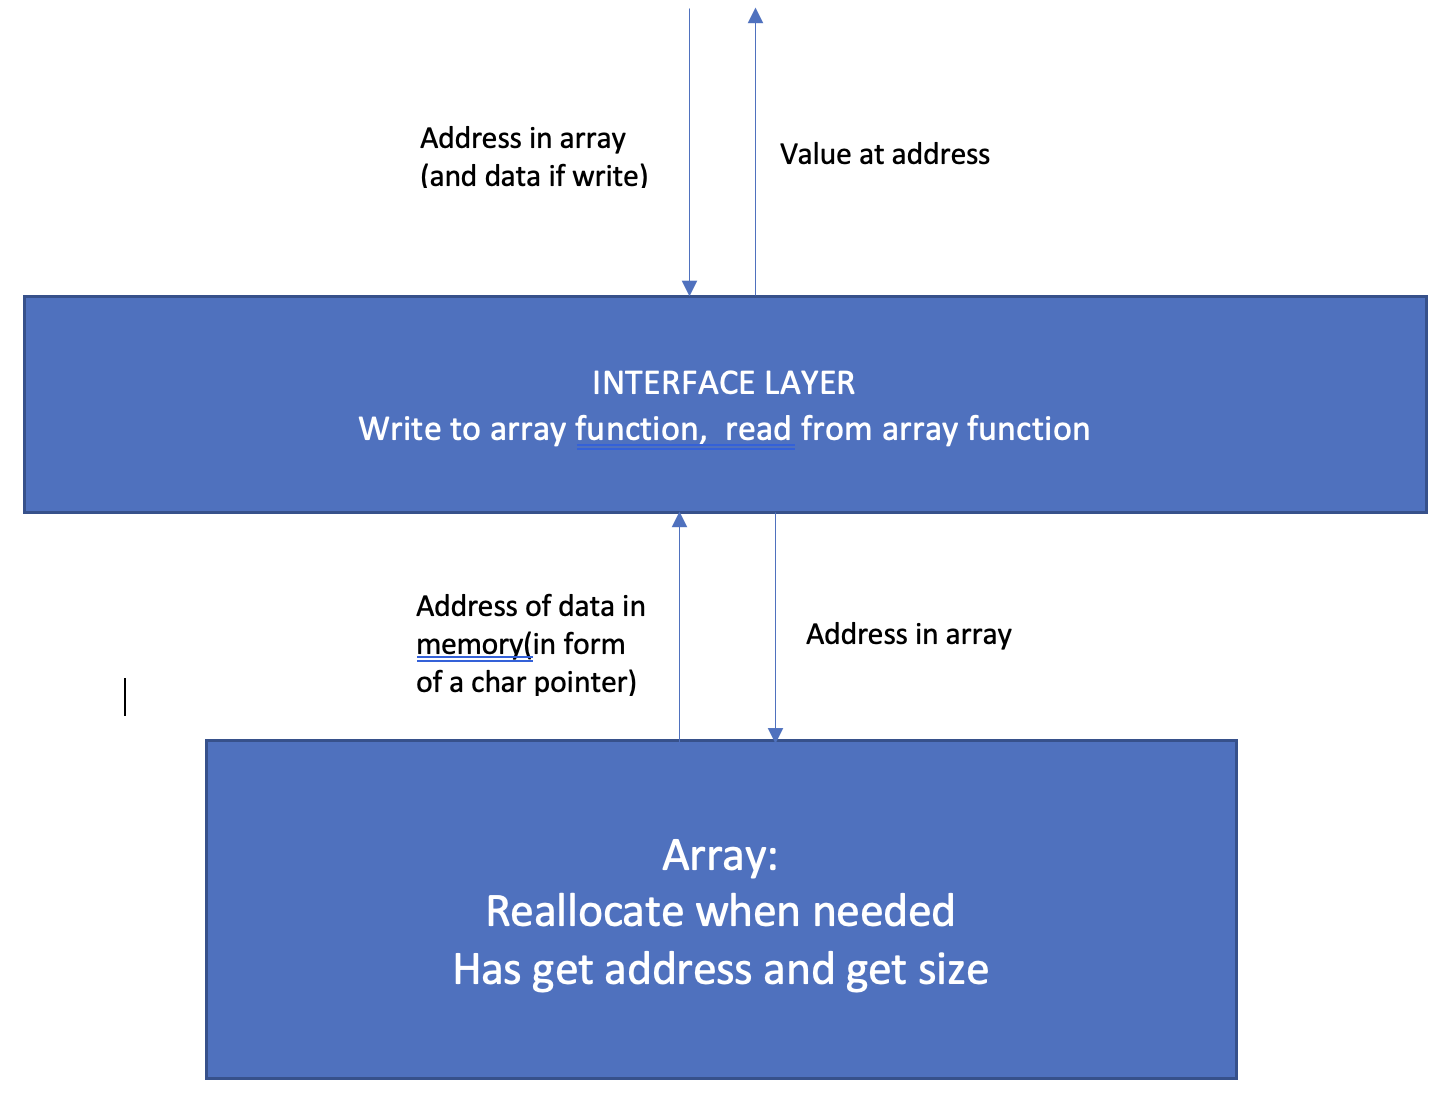
\includegraphics[width = \linewidth]{ mem_array }
\caption{Encapsulated structure of the polymorphic memory array}
\label{fig:mem_array}
\end{minipage}
\end{figure}

\subsubsection{First pass: Parser and Tokenizer}
In the first pass, the assembly file was read line by line until the end of the file. The number of words in each line was kept track of. If there was only one word in a line, that line would be a label. If so, the label would be added to the symbol table. If the line was a normal instruction instead, then the opcode and operands would be stored inside a singly linked list representing the disassembled lines.
\subsubsection{Second pass}
In the second pass, the linked list of disassembled lines was processed recursively. Each line was mapped to the corresponding translate function pointer and a default condition binary code. The function is then executed to produce the required binary. This made the functions more independent and made it easier to carry out function testings.
    
\subsubsection{Translate functions}
Similar to the emulator, the assembly lines and the respective functions are categorized into 4 main types: data process, data transfer, multiply and branch, and function pointers were applied as well.  There were several similarities in how different categories of lines are decoded so helper functions were created to reduce code duplication.

\subsubsection{Output}
The binary lines would then be converted to little-endian format and printed out into the output file.

\subsection{Challenges}
A problem was choosing the appropriate form of data representation for assembly lines. The original method was to use a dynamic array like the memory array that was implemented early on. This required the assembly lines to be looped through twice which reduced efficiency. We got around this by using the linked list. Even though a linked list complexity is higher than a static array, the assembly lines are read sequentially, which makes the execution time similar to a static array.\newline
For the symbol table, we used the memory array data structure from the emulator because:
    
1. The size of the array is unknown, which could be solved with the memory array's internal reallocation function.
    
2. Memory array can be used to store any type of element. The type conversion would be defined at the interface shown in Figure 2.
\pagebreak
\section{Extension: Three-player Chess}
The theme chosen for the extension part of the project is a three-player chess game played on a hexagonal, 96-tile chessboard. Although there are many variants involving different shapes of boards and rules, the most straightforward and regular-chess-like rules are selected.
\subsection{Game Design}
\subsubsection{Board layout}
As shown in Figure 3, the board can be divided into 3 sections with the size of 8 rows * 4 columns, which are assigned to the three players' colours black, white and red. The tiles can be labelled with a combination of 12 numbers and 8 letters, just like regular chess. The initial state for one side of the board is the same as in regular chess.
\subsubsection{Rules}
The rules generally follow from regular chess, whenever a piece is considering moves within the three 8*4 areas mentioned in 3.1.1, the possible moves are the same as in regular chess. Therefore, castling and promotions are also possible. The difference is when the piece attempts to cross the "rosette tiles" located at the centre of the board (d4, e4, d5, i5, i9, e9) and the "side" tiles (on rows 4, 5, 9, including the rosette tiles). Two additional rules are accounting for these kinds of movements:

1. When a piece on the rosette tiles is considering moving on the diagonal line towards the board centre, the diagonal path would divert into two, or more specifically, continues on the two tiles with the same colour;

2. When a piece on the side tiles is considering moves on the vertical line or diagonal line towards the distorted edge, the direction diverts to the nearest side tile (with the same colour if diagonal) and continues from there on.

Hence, as shown in Figure 4, the left king's diagonal movement towards the board centre will be diverted into two directions, and the vertical movement and diagonal movement towards the left 8*4 area will land on the nearest tile with a different colour and an identical colour respectively. These two rules apply to all pieces.

\begin{figure}
\centering
\begin{minipage}{.5\textwidth}
\centering
\includesvg[width = \linewidth]{ board }
\caption{Hexagonal chessboard}
\label{fig:board}
\end{minipage}\hfill
\begin{minipage}{.5\textwidth}
\centering
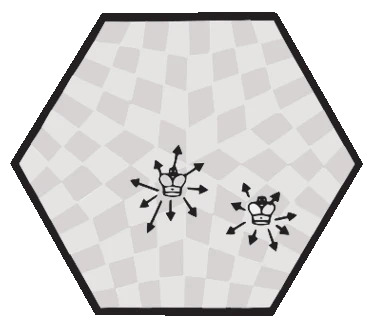
\includegraphics[width = \linewidth]{ king_moves }
\caption{Possible moves for King}
\label{fig:moves}
\end{minipage}
\end{figure}

\subsubsection{Legal Moves}
Following the rules, the moves generated are in a stage called pseudo-legal move. What differentiates them from actual legal moves is that legal moves would never put their king in check after the move has commenced.
\subsubsection{Objective for the Game}
The main objective for the three players will still be the first to checkmate another player, that is, to pin down the opponent's king in a situation in which no legal move is available to the opponent. Once the game is in a state of checkmate (as well as draw, which can be voted as an end-game option mid-game, or stalemate, meaning that a player has no legal move without being checked) it will then conclude, and 1 point will be added to the winning player.\newline
\begin{figure}
\begin{minipage}{.5\textwidth}
\ centring
\includegraphics[scale = 0.3]{ chess_communication_structure }
\caption{Possible moves for King}
\label{fig:moves}
\end{minipage}
\end{figure}
\subsection{Code structure}
\subsubsection{Board Logic}
The Board Logic code manages the board state, checks and processes legal piece moves, generate available moves during the process and maintains the game state. After initialising the memory and board state, the game starts with the white player and loops through the order of red, black and white. It will first check for game state and decide if the game proceeds or concludes. Then, for every click on an ally piece, the available moves are produced and sent to the GUI for rendering and checks for another click on the available tiles. If the second click is on the available tiles, it will then process the move and check for castling and promotion.\newline
The algorithm for generating available moves generally follows from 3.1.2, with the usage of vectors to generate all moves in a loop. Using this algorithm, the program can check for king checks simply by generating all enemy pieces' moves and matching them with the ally king's coordinates. Similarly, legal moves are checked by plugging the modified board with the pseudo-legal move commenced.
\subsubsection{GUI Design}
The second part is the GUI design which is done in Unity Engine. It includes the rendering of the chessboard model mentioned before, as well as the chess pieces in three colours and the tile colour change when showing available moves, whenever a player clicks on any piece. As well as this, there is a menu system with variables managed only in Unity that personalise the game such as the names of the individual player that had no need to be handled or sent to the other sides
\subsection{Socket connection}
Since the unity engine only supports c#, a way of communication need to be established between the GUI and the board logic. Read and write to file was the initial idea however due to its inability to have a consistent update, that idea was discarded. The final idea was to use socket transmission. Since c contains low-level language features, this gives more flexibility when designing network transmission. For the GUI logic communication, a server was set up at the beginning of the program and the GUI set up a client socket using the localhost IP(127.0.0.1) and start the connection. The detail of the communication is shown in figure 5.\newline
An attempt was given for setting up a LAN(local area network)lobby room, by asking the client to broadcast a unique message, while the host listens to the port, this allows the host to find out the client's IP address. The host can then send a direct datagram allowing the client to discover the host IP address and request for connection. However, due to time constrain, this could not be implemented.
\pagebreak
\section{Reflections}
\subsection{Group Reflection}
The team collaboration was smooth and efficient throughout the process. From splitting our work evenly and dividing the independent works into different files, to communicating through Discord, tracking progress on Trello, and organising offline meetings and coding sessions, every member is always on the same page and working on different things. Although there are hiccups in between the planning stage and coding stage for the extension concerning the use and learning progress of the GTK+ library, in general, every member contributed to many parts of the project, and the progress made is all crucial to the final product.
\subsection{Individual Reflections}
\subsubsection{Andy Chen}
\subsubsection{HouWang Wong}
During the first stage, as I have had quite a bit of experience with the C language before, I could quickly complete my parts and started debugging and implementing additional features. However, for the second part, I have to admit that I misjudged the time necessary for me to learn the GTK+ library, let alone the limits of the library when compared to the Unity Engine and other game design engines. Despite that, I completed the refinement of both reports, presentation slides and scripts, which I am experienced with. This experience will remind me in further projects to carefully assess my capabilities and the time limit before planning.
\subsubsection{Jeshuran Jebanesan}
I took over the GUI using Unity. I think I may have been too ambitious and not fully understood the scope of what I was doing. In the future, I should aim to create a base version of the program before going on to add extensions to the game. I could have done this in our project by mapping the project to 3 4 by 8 arrays in C first. In our game, I tried to deal with castling, promotions and other special niche cases and menu interactions before finishing the base rules. However, at the same time, I was able to learn a lot to do with Unity, and sockets and I appreciated the team I was with and the importance of morale. Completing functions which had taken a long time resulted in a cheer from everyone even if they didn't know what code was completed.
\subsubsection{Jiaju Yang}
Previously I have some experience in c++, which helped me with understanding accessing memory with a pointer. However all pointers in c are manually managed and this caused me some confusion on using the correct data type and operation to interact with the data, for example between using memory move and just passing by pointers. Through debugging the assembler, I was able to learn how each data structure affects the memory and avoid the misuse of data structures. During extension, I got the opportunity to research socket communication in c which is an area I never touched on. This gives me more flexibility when designing and coding future projects. On the other hand, due to the lack of experience in project planning, for example, the amount of workload and the planning of testings of the sub-function lead to more time lost due to debugging.
\end{document}
